\documentclass[11pt]{beamer}
\usetheme{Madrid}
\usepackage[utf8]{inputenc}
\usepackage[french]{babel}
\usepackage[T1]{fontenc}
\usepackage{amsmath}
\usepackage{amsfonts}
\usepackage{amssymb}
\usepackage{graphicx}

\author{Fehr Mathieu, Pluvinage Lucas, Voss Malachi, Dang-nhu Hector}
\title{Projet Système Digital}


\begin{document}

\begin{frame}
\titlepage
\end{frame}


\section{Plan de la presentation}

\begin{frame}{Plan de la présentation}
\begin{itemize}
\item Compilateur de netlists
\item Amélioration de minijazz
\item Ajout d'affichages en parallèle
\item Architecture du processeur
\item Instructions assembleurs
\item Création de la montre
\end{itemize}
\end{frame}


\section{Compilateur de netlists}
\begin{frame}{Compilateur de netlists}
Spécifications du compilateur :
\begin{itemize}
\item{Codé en C++ en utilisant lexertl}
\item{Code les netlists en C++0x}
\item{Les fils sont codés sur des booléens, et les nappes de fils sont codés sur
  des entiers (8,16,32 ou 64 bits)}
\item{Généralisation des opérations binaire sur les nappes de fils (possibilité
    d'effectuer toutes les opérations en moins de 2 cycles processeur)}
\item{Gestion de la ram via des tableaux statiques}
\end{itemize}
\end{frame}


\section{Amélioration de minijazz}

\begin{frame}{Amélioration de minijazz pour notre simulateur}
  Minijazz a été modifié pour permettre l'utilisation des opérations suivantes :
  \begin{itemize}
  \item{Les opérations binaires sur plusieurs bits}
  \item{avoir un multiplexeur dont les sorties se font sur plusieurs bits}
  \end{itemize}

  Ces changement permettent de réduire énormément la taille de notre netlist produite.
\end{frame}

\section{Affichage en parallèle}

\begin{frame}{Affichage en parallèle}
  Pour pouvoir afficher les sorties du simulateur autrement qu'en console (ce
  qui réduit énormément la vitesse d'éxecution), nous avons modifié le
  simulateur pour pouvoir intégrer en son code des bouts de codes C++,
  permettant d'afficher certaines de ces variables.
  
  Un tel affichage a été utilisé pour la montre, par la SDL dans un thread séparé.
\end{frame}

\begin{frame}{Architecture du processeur}
  Le processeur suit une architecture 32 bits ARM. Il implémente les opérations
  logiques et arithmétiques de bases, ainsi que le barrel pour toutes les
  opérations.
  Il est composé des blocs suivants :
  \begin{itemize}
  \item{L'ALU, effectuant les calculs et méttant à jour les flags}
  \item{Le barrel shifter, permettant de faire des shifts et des rotations}
  \item{Le test de conditionnement, qui vérifie si l'opération en cours doit
      être executé}
  \item{la gestion de la mémoire RAM/ROM, qui gère aussi les registres}
  \item{Le sélecteur d'instruction, qui regarde quelle opération effectuer}
  \end{itemize}
  Le processeur contient en tout environ 3000 portes, dont beaucoup sont
  optimisées par gcc.
\end{frame}

\begin{frame}
    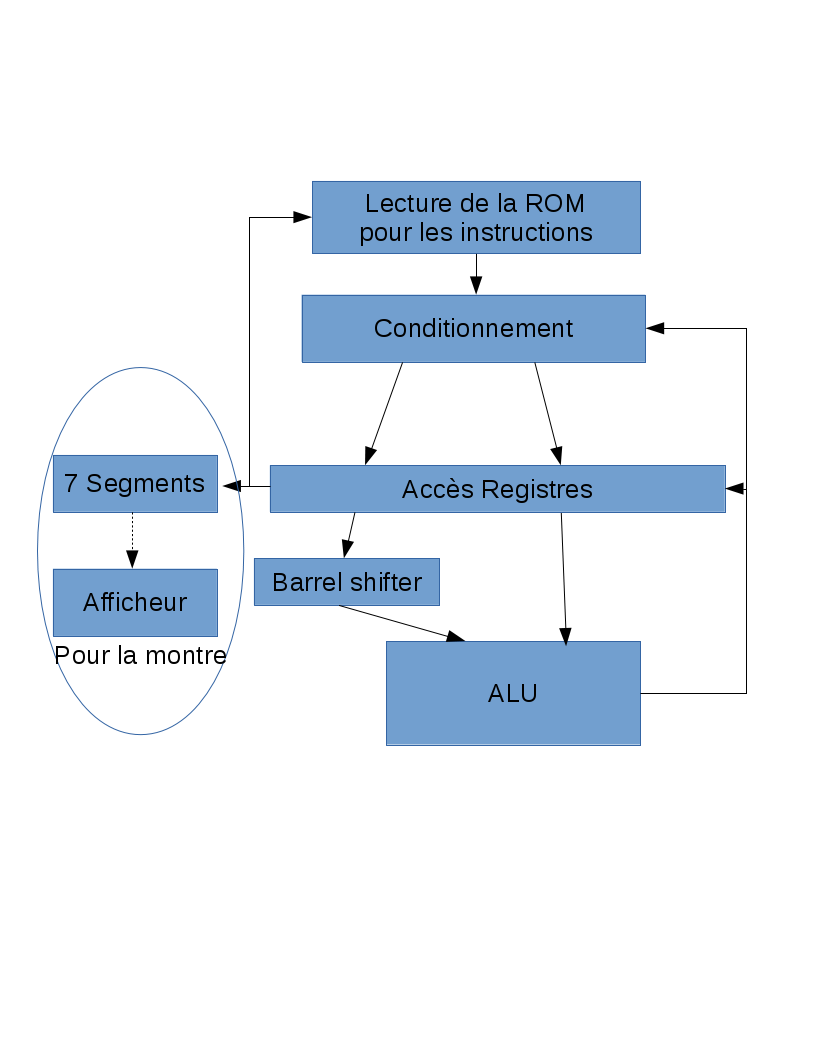
\includegraphics[scale=0.4]{test.png}
\end{frame}

\begin{frame}{Instructions assembleurs}
  Les instructions assembleurs sont celles des processeurs ARM, avec en plus
  deux ajouts. Elles sont écrites sur 32 bits, et sont structurées ainsi :
  {\tiny
  \begin{tabular}{|c|c|c|c|c|c|c|c|c|c|c|c|}
  \hline
  0-3  & 4 & 5 & 6 & 7 & 8-10 & 11 & 12-15 & 16-19 & 20-23 & 24-27 & 28-31 \\
  \hline
  COND & 0 & 0 & I & \multicolumn{2}{c|}{OPCODE} & Set flag & Registre rd & Registre op1 & \multicolumn{3}{c|}{Opérande op2}  \\
  \hline
  COND & 0 & 0 & 1 & \multicolumn{2}{c|}{OPCODE} & Set flag & Registre rd &Registre op1 & Shift & \multicolumn{2}{c|}{Constante} \\
  \hline
  COND & 0 & 0 & 0 & \multicolumn{2}{c|}{OPCODE} & Set flag & Registre rd & Registre op1 & \multicolumn{2}{c|}{Shift} & r2  \\
  \hline
  COND & 1 & 0 & 1 & linking & \multicolumn{ 7}{c|}{Offset} \\
  \hline
  COND & 1 & 1 & 1 & 0 & \multicolumn{4}{c|}{Port} & \multicolumn{3}{c|}{Valeur} \\
  \hline
  \end{tabular}}
L'utilisation de op2 permet d'avoir des constantes plus grandes que 8 bits.
\end{frame}

\begin{frame}{Création de la montre}
  La montre est écrite en ARM, et n'utilises que les opérations ADD, MOV, B, BL
  et WAI. La montre est écrite en deux versions :
  \begin{itemize}
  \item{Une pouvant être synchronisé aux secondes grace a la lecture d'une
      horloge interne, synchronisée à l'ordinateur}
  \item{Une itérant le plus rapidement possible les secondes, pouvant de cette
      manière parcourir quelques jours en une seconde}
  \end{itemize}
\end{frame}

\begin{frame}{Explication du programme}
  Les unités de temps ne sont jamais stockées en binaire sur des registres. A la
  place, on stocke les digits en binaire. Cela permet d'afficher simplement les
  digits.\\

  r0 : 
  \begin{tabular}{|c|c|c|c|c|c|c|c|c|c|c|}
    \hline
    1 & 1 & 4 & 2 & 4 & 2 & 4 & 3 & 4 & 3 & 4\\
    \hline
    inutilisé & \multicolumn{2}{c|}{mois} & \multicolumn{2}{c|}{jours} & \multicolumn{2}{c|}{heures} & \multicolumn{2}{c|}{minutes} & \multicolumn{2}{c|}{secondes} \\
    \hline
  \end{tabular}

  r1 :
  \begin{tabular}{|c|c|c|c|c|c|}
    \hline
    2 & 14 & 4 & 4 & 4 & 4\\
    \hline
    années modulo 4 & inutilisé & \multicolumn{4}{c|}{années} \\
    \hline
  \end{tabular}
 
  \begin{itemize}
  \item Les registres r2...r6 sont utilisé pour stocker des constantes accélérant les
  calculs, et les registres r7...rE sont utilisés comme pointeurs.\\

  
  \item Le programme fonctionne par blocs de niveaux, permettant de ne pas avoir à
  vérifier combien de jours une année possède par exemple.\\

  
  \item Cette méthode de fonctionnement permet de modifier tous les digits (sauf les
  années) en une instruction.
  \end{itemize}
\end{frame}

\end{document}
